\chapter{PySPH and DEM}

The Discrete Element Method, being a particle method, has attributes which allow for an implementation in the PySPH framework. These attributes, introduced in section \ref{sec:DEM}, are:

\begin{itemize}
\item Representation of the Solid Bodies as ``particles''.
\item Efficient search of particles coming into contact with one another via Boxing and Contact Searching.
\end{itemize}

In PySPH, the solid bodies can be represented as a collection of particles assigned with a ``body tag'' to demarcate the individual solid entities. Further, for neighbour search, the hypersphere of influence is analogous Boxing. Lastly, contact can then be established by using contact models and the contact forces can be computed. Thus, conceptually, a DEM implementation in PySPH should be possible.

This chapter describes a Soft Contact model and it's PySPH implementation. Thereafter, a case study performed to validate the collision model is described. Finally, the conclusions of the validation study are presented.

\section{Validation of the RigidBodyCollision Model}

This model \cite{gpu_gems}\footnote[8]{\url{http://http.developer.nvidia.com/GPUGems3/gpugems3_ch29.html}} represents the Proof of Concept establishing that DEM can be implemented in PySPH. It models the contacts as a Spring and Dashpot system as follows:

\begin{eqnarray}\label{eq:RigidBodyCollision}
Repulsive Force, f_{i,s} &=& -k~(d-|{\bf{r_{ij}}}|)~\frac{{\bf{r_{ij}}}}{|{\bf{r_{ij}}}|} \nonumber\\
Damping Force, f_{i,d} &=& \eta ~ {\bf{v_{ij}}} \\
Shear Force, f_{i,t} &=& k_{t}~{\bf{v_{ij,{\it{t}}}}} \nonumber
\end{eqnarray}

{\raggedright{where},} \\
{\it{k}} $=$ Spring Coefficient $\hspace{0.375cm}$ ; $\hspace{0.375cm}$ {\it{k$_t$}} $=$ Coefficient of Shear $\hspace{0.375cm}$ ; $\hspace{0.375cm}$ $\eta =$ Damping Coefficient\\
d $=$ diameter of elements comprising the body\\ 
${\bf{r_{ij}}} = \textbf{r}_{i} - \textbf{r}_{j}$ $\hspace{0.375cm}$ ; $\hspace{0.375cm}$ ${\bf{v_{ij}}} =\textbf{v}_{i} - \textbf{v}_{j} $ \\
Relative Tangential Velocity, ${\bf{v_{ij,{\it{t}}}}} = {\bf{v_{ij}}} - \left({\bf{v_{ij}}} \cdot \frac{{\bf{r_{ij}}}}{|{\bf{r_{ij}}}|}\right) \frac{{\bf{r_{ij}}}}{|{\bf{r_{ij}}}|} $\\

In order to validate the RigidBodyCollision Model, a comparison with experimental results published by \cite{zhang} is made. The experimental set up consisted of an acrylic resin tank with dimensions of 26 cm $\times$ 10 cm $\times$ 26 cm (L$\times$B$\times$H) with solid aluminium cylinders of diameter 1 cm, length 9.9 cm, and density 2.7 $\times$ 10$^3$ $\frac{kg}{m^3}$ stacked in horizontal layers as shown in Figure \ref{fig:exp_setup}. The system is held in equilibrium by a plate which is removed to begin the experiment. The state of the system for a 6 layer cylinder stack (Figure \ref{fig:sys_state}) is captured using a High Speed camera shooting at 200 frames per second. Also, the evolution of the average mass centers of the six cylinder collapse is plotted (Figure \ref{fig:sys_cm}) after 5 experimental trials.

\begin{figure}[htb!]
\centering
\setlength\fboxsep{0pt}
      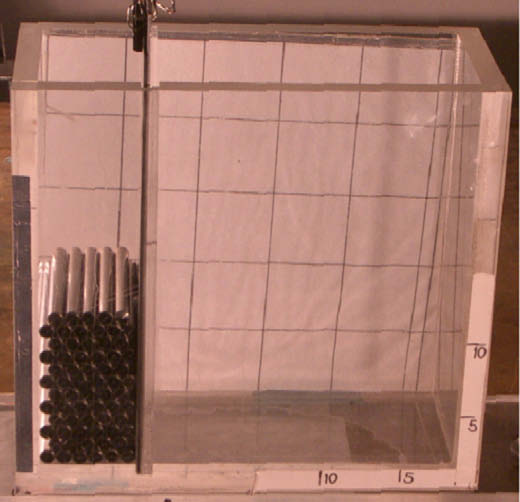
\includegraphics[scale=0.3]{figures/exp_setup.png} 
\caption{{\small{Experimental Setup}}}
\label{fig:exp_setup}
\end{figure}

\begin{figure}[htb!]
\centering
\setlength\fboxsep{0pt}
      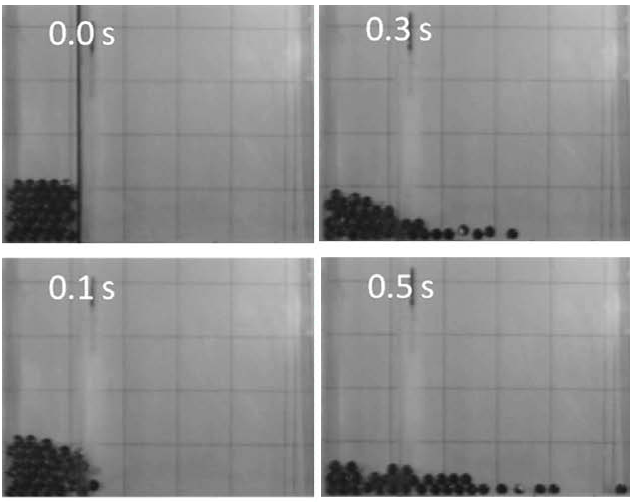
\includegraphics[scale=0.3]{figures/sysEvol.png} 
\caption{{\small{Evolution of 6 Cylinder Stack}}}
\label{fig:sys_state}
\end{figure}

\begin{figure}[htb!]
\centering
\setlength\fboxsep{0pt}
       \begin{tabular}{cc}
 	   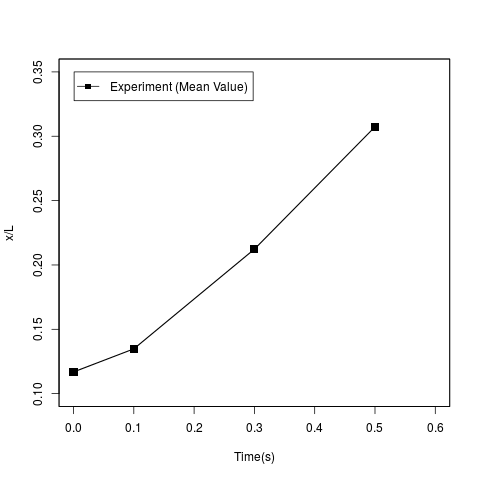
\includegraphics[scale=0.325]{figures/XexpDataR.png} &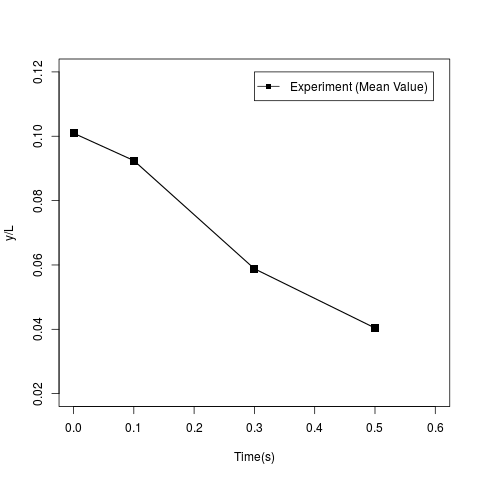
\includegraphics[scale=0.325]{figures/YexpDataR.png}
 	   \end{tabular}      
\caption{{\small{Six Cylinder System Center of Mass (x, y are the center of masses in the X and Y directions)}}}
\label{fig:sys_cm}
\end{figure}

The ~ 6 ~ cylinder ~ case ~ is ~ set ~ up ~ in ~ PySPH ~ via ~ the ~ ``\_create\_geometry.py'' ~ and the ``rigid\_body\_validation.py'' (\ref{app1:case}) programs respectively. The particles are created using the \lstinline!create_particles()! method in the \lstinline!class CollapsingCylinderGeometry()!, the solver is created using \lstinline!create_solver()! method and the interaction physics is defined in the \lstinline!create_equations()! method, from the \lstinline!class CollapsingCylinder()!; a body force of 981 $\frac{cm}{s^2}$ is imparted in the $-Y$ direction, collisions are modelled and Newton's Equations for Rigid Body Dynamics (Equation \ref{eq:newton}) are solved.

\begin{eqnarray}\label{eq:newton}
Rigid Body ~{\textit{\textbf{I}}} &=& \left\lbrace particles : r_{ij} = 0, ~ \forall t , i,j \in I\right\rbrace \nonumber \\
M_{I}\frac{d{\it{{\bf{V_I}}}}}{dt} &=& \sum_{k~\in~I} m_{k} \frac{d{\it{{\bf{v_k}}}}}{dt} \\
{\bf{\it{I_I}}} \frac{d{\bf{\varOmega _{I}}}}{dt} &=& \sum_{k~\in~I} m_{k}\left( {\bf{r_k - R_I}}\right) \times \frac{d{\it{{\bf{v_k}}}}}{dt} \nonumber
\end{eqnarray}

{\raggedright{where,}} \\
$M_I , {\it{\bf{V_I}}}, {\it{\bf{R_I}}} = $ Mass, Velocity and Center of Gravity of {\it{``I''}}, \\
$I_I , {{\bf{\varOmega _{I}}}} = $Inertial Tensor(Moment of Inertia), Angular Velocity of {\it{``I''}} \\
$m_k , {\it{{\bf{v_k}}}}, \bf{r_k} =$ Mass, Velocity and Position of $k^{th}$ particle\\

The case set up in PySPH is shown in Figure \ref{fig:sim_setup}. Among the various parameter combinations tried, the best results were obtained for the parameter values of $k = 8.0, d = 2.5, \eta = 0.01$ and $k_t = 0.1$. However, a qualitative inspection of the simulation shows that the model is physically inconsistent. A snapshot of the simulation at time $t = 0.032s$ is shown in Figure \ref{fig:bestresult_snapshot} where the cylinder arrays can be seen to merge into one another. A possible explanation for the failure of the model could be that there is no description of the material properties of the interacting solid bodies which would definitely play a vital role in the collision process. This observation leads us to move on to the search of a better suited model, which is further detailed in the next chapter.

\begin{figure}[htb!]
 \begin{subfigure}{.5\textwidth}
  \centering
    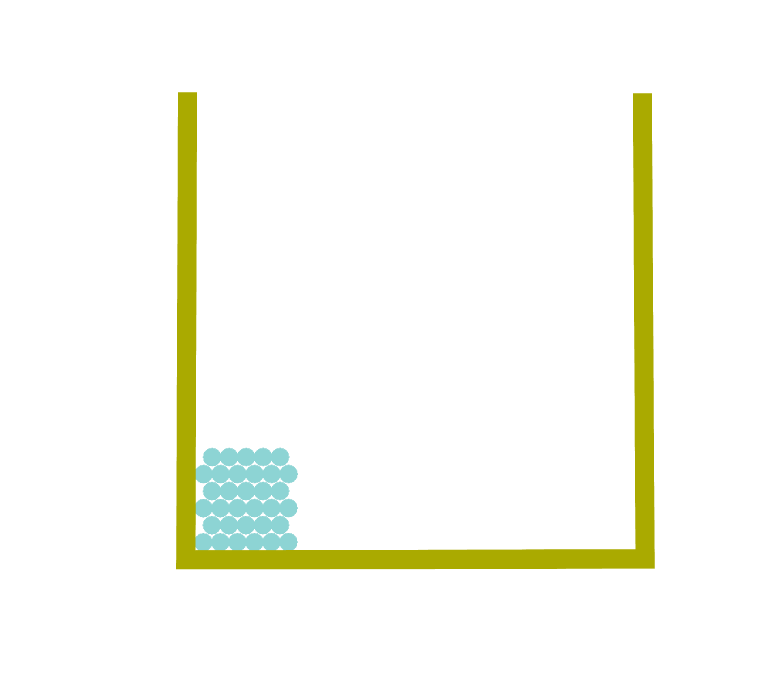
\includegraphics[width=.94\linewidth]{figures/setup.png} 
    \caption{{\small{Case set up in PySPH}}}
    \label{fig:sim_setup}
 \end{subfigure}
 \begin{subfigure}{.5\textwidth}
  \centering
    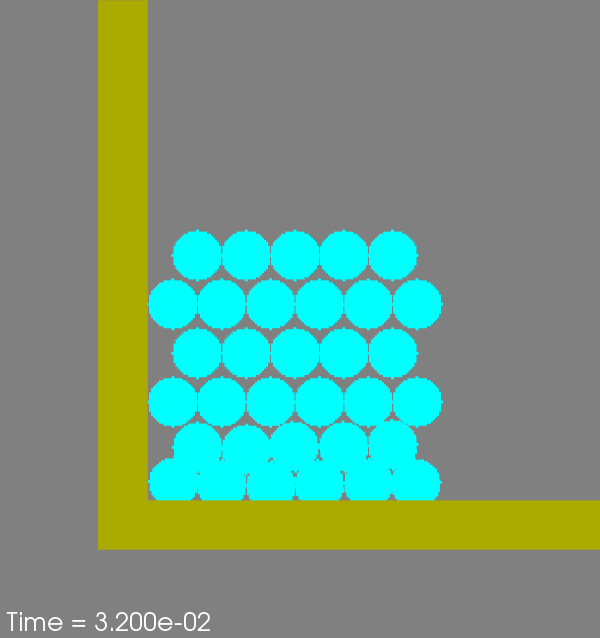
\includegraphics[width=.8\linewidth]{figures/frame000031.png}
    \caption{{\small{System State at time, $t = 0.032 s$}}}
    \label{fig:bestresult_snapshot}
 \end{subfigure}
 \caption{PySPH Validation Study}
\end{figure}